% ****** Start of file apssamp.tex ******
%
%   This file is part of the APS files in the REVTeX 4.1 distribution.
%   Version 4.1r of REVTeX, August 2010
%
%   Copyright (c) 2009, 2010 The American Physical Society.
%
%   See the REVTeX 4 README file for restrictions and more information.
%
% TeX'ing this file requires that you have AMS-LaTeX 2.0 installed
% as well as the rest of the prerequisites for REVTeX 4.1
%
% See the REVTeX 4 README file
% It also requires running BibTeX. The commands are as follows:
%
%  1)  latex apssamp.tex
%  2)  bibtex apssamp
%  3)  latex apssamp.tex
%  4)  latex apssamp.tex
%
\documentclass[%
 reprint,
%superscriptaddress,
%groupedaddress,
%unsortedaddress,
%runinaddress,
%frontmatterverbose, 
%preprint,
%showpacs,preprintnumbers,
%nofootinbib,
%nobibnotes,
%bibnotes,
 amsmath,amssymb,
 aps,
%pra,
%prb,
%rmp,
%prstab,
%prstper,
%floatfix,
]{revtex4-1}

\usepackage{graphicx}% Include figure files
\usepackage{dcolumn}% Align table columns on decimal point
\usepackage[spanish]{babel}
\selectlanguage{spanish} 
\usepackage[utf8]{inputenc}
\usepackage{bm}% bold math
%\usepackage{hyperref}% add hypertext capabilities
%\usepackage[mathlines]{lineno}% Enable numbering of text and display math
%\linenumbers\relax % Commence numbering lines
\usepackage{float}
%\usepackage[showframe,%Uncomment any one of the following lines to test 
%%scale=0.7, marginratio={1:1, 2:3}, ignoreall,% default settings
%%text={7in,10in},centering,
%%margin=1.5in,
%%total={6.5in,8.75in}, top=1.2in, left=0.9in, includefoot,
%%height=10in,a5paper,hmargin={3cm,0.8in},
%]{geometry}
\usepackage[font=footnotesize,labelfont=bf]{caption}
\usepackage{hyperref}
\newcommand{\subtitle}[1]{%
\posttitle{%
    \par\end{center}
\begin{center}\large#1\end{center}
\vskip0.5em}%
}
\begin{document}

%\preprint{APS/123-QED}

\title{Efecto Hall\\ \textit{Estudio de efectos clásicos y cuánticos } }% Force line breaks with \\

%\subtitle{Estudio de la dualidad de onda partícula}

\author{Jose Alejandro Montaña Cortés}
\email{ja.montana@uniandes.edu.co}
% \altaffiliation[Also at ]{Departamento de Física, Universidad de los Andes}
\author{Jesús David Rincón Puche}%
\email{jd.rincon883@uniandes.edu.co}
\affiliation{Departamento de Física, Universidad de los Andes}%

%\collaboration{}%\noaffiliation

\date{\today}% It is always \today, today,
             %  but any date may be explicitly specified

\begin{abstract}

En este experimento se realizaron medidas para el efecto Hall clásico sobre una placa semiconductora tipo P de germanio puro. Primero se realizó una calibración del campo magnético que actúa sobre la placa, encontrando que aproximadamente 1 $A$ equivale a 200 $mT$. Seguido de esto, se realizaron medidas del voltaje Hall ($V_H$) en función de la corriente paralela ($I_p$) y se encuentra exitosamente el comportamiento lineal esperado; en adición,se observó que al agregar campo magnético el valor de la resistencia de Hall ($R_H$) disminuye, gracias al aumento en $V_H$. En la tercera parte, se realizó un experimento para observar la magnetoresistencia, fenómeno en el cual una resistencia eléctrica aumenta gracias a un campo magnético aplicado, sin mucho éxito por posibles daños en la placa semiconductora. Finalmente, se desarrolló un experimento para observar como la conductividad disminuye con la temperatura, obteniendo resultados deseados para este experimento.

\end{abstract}
\maketitle
%\tableofcontents

%---------------------INTRODUCCIÓN------------------
\section{Introducción}

 
 
 \section{Desarrollo Teórico}
 
 \subsection{Efecto Zeeman}
 

% trim={<left> <lower> <right> <upper>}
%----MONTAJE EXPERIMENTAL--------
\section{Montaje experimental}
\subsection{Instrumento de medición.}


%-----------------RESULTADOS----------------------
\section{Resultados y Análisis}
\subsection{Relación entre la corriente que pasa por el montaje y el campo magnético generado}
Dado que el Teslámetro que se tenía a disposición era un aparato sensible y delicado, se empezó primero por caracterizar como se comportaba el campo magnético generado por las bobinas en función de la corriente que circulaba por estas. Esto con el fin de que cuando se hablara de campo magnético, se supiera su equivalente en terminos de la corriente y así con esto minimizar el uso del aparato.\\
Tal y como se muestra en la figura \ref{Calibracion}, la relación entre la corriente que circula por las bobinas y el campo magnético es de tipo lineal. Con esto se tiene entonces que hablar de corriente es equivalente a hablar de campo magnético\footnote{Es por esto que de ahora en adelante cuando se hable de campo magnético sus unidades serán Amperios}.

\begin{figure}[h]
\center{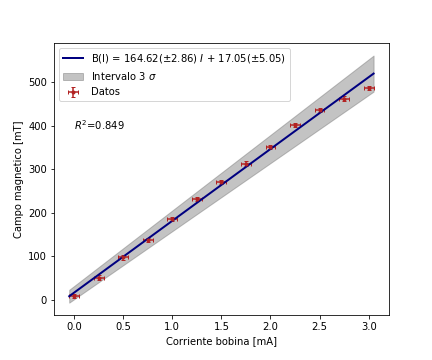
\includegraphics[width=0.4\textwidth]
{../Figuras/Calibracion_error.png}}
\caption{\label{Calibracion}. Gráfico del campo magnético medido por el Teslametro en función de la corriente suministrada por la fuente. La linea en azul corresponde al ajuste efectuado, a los datos experimentales y la región sombreada corresponde a los intervalos de confidencia con $5\sigma$}
\end{figure}

\subsection{Determinación de la resistencia de Hall.}
Una vez caracterizado el campo magnético en función de la corriente, se fijó el campo magnético en 1.5 A y se analizó el comportamiento entre el voltaje de Hall $V_H$ en función de la corriente que pasaba por el material $I_p$
\begin{figure}[h]
\center{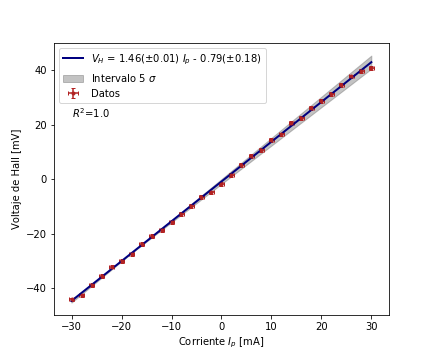
\includegraphics[width=0.4\textwidth]
{../Figuras/Voltaje_hall_ip.png}}
\caption{\label{V_H_vs_I_p}.  La linea en azul corresponde al ajuste efectuado, a los datos experimentales y la región sombreada corresponde a los intervalos de confidencia con $5\sigma$}
\end{figure}

\begin{figure}[h]
\center{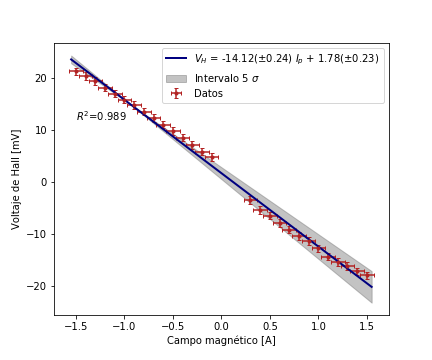
\includegraphics[width=0.4\textwidth]
{../Figuras/Voltaje_hall_Campo_magnetico.png}}
\caption{\label{V_H_vs_campo}.  La linea en azul corresponde al ajuste efectuado, a los datos experimentales y la región sombreada corresponde a los intervalos de confidencia con $5\sigma$}
\end{figure}

\begin{figure}[h]
\center{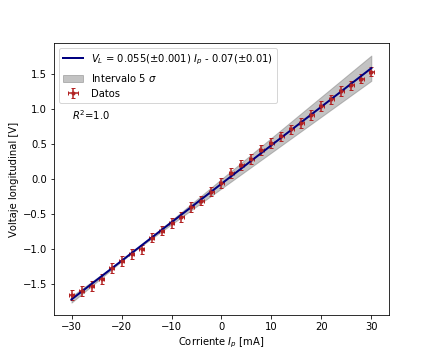
\includegraphics[width=0.4\textwidth]
{../Figuras/Voltaje_longitudinal_ip.png}}
\caption{\label{V longitudinal vs ip}.  La linea en azul corresponde al ajuste efectuado, a los datos experimentales y la región sombreada corresponde a los intervalos de confidencia con $5\sigma$}
\end{figure}

\begin{figure}[h]
\center{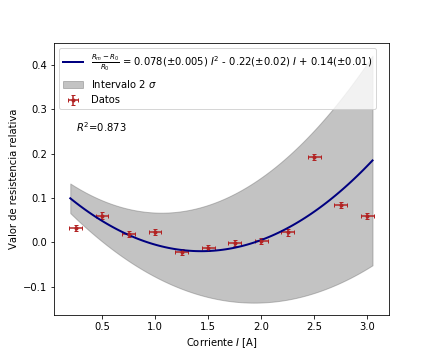
\includegraphics[width=0.4\textwidth]
{../Figuras/Resistencia_vs_Campo_magnetico.png}}
\caption{\label{R_vs_Campo}.  La linea en azul corresponde al ajuste efectuado, a los datos experimentales y la región sombreada corresponde a los intervalos de confidencia con $5\sigma$}
\end{figure}



\begin{figure}[h]
\center{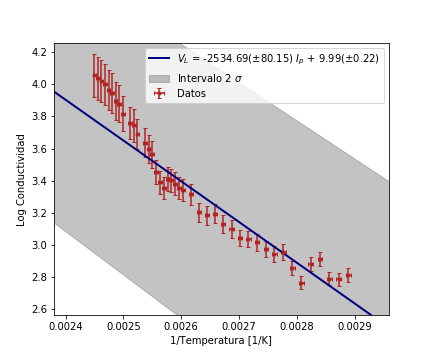
\includegraphics[width=0.4\textwidth]
{../Figuras/Comnductividad_Temperatura.png}}
\caption{\label{Conductividad en función de la temperatura}.  La linea en azul corresponde al ajuste efectuado, a los datos experimentales y la región sombreada corresponde a los intervalos de confidencia con $5\sigma$}
\end{figure}


\begin{figure}[h]
\center{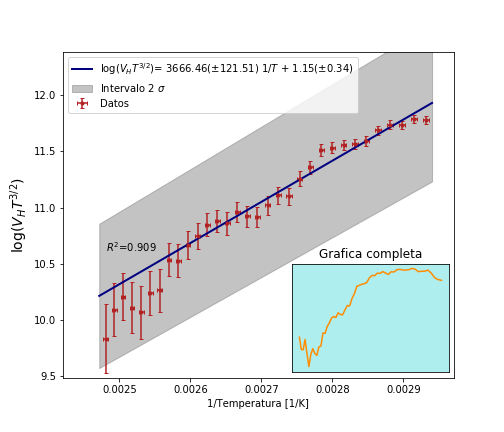
\includegraphics[width=0.4\textwidth]
{../Figuras/Region_intrinseca.png}}
\caption{\label{Region intrinseca}.  La linea en azul corresponde al ajuste efectuado, a los datos experimentales y la región sombreada corresponde a los intervalos de confidencia con $5\sigma$}
\end{figure}


\begin{figure}[h]
\center{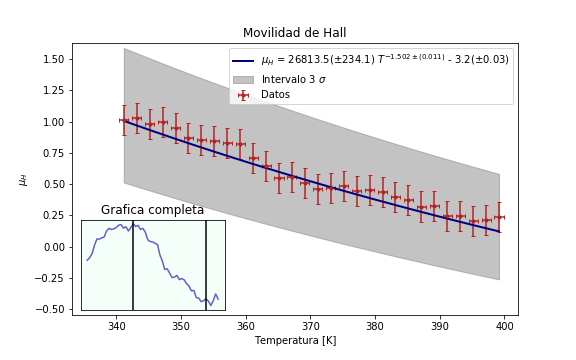
\includegraphics[width=0.4\textwidth]
{../Figuras/Movilidad_Hall.png}}
\caption{\label{movilidad de Hall}.  La linea en azul corresponde al ajuste efectuado, a los datos experimentales y la región sombreada corresponde a los intervalos de confidencia con $5\sigma$}
\end{figure}
%---------------CONCLUSIONES-------------------

\section{Conclusiones}
\begin{itemize}
    \item 
    \item 
\end{itemize}
%Se deben contestar las preguntas planteadas inicialmente o dar las razones por las cuales no es posible hacerlo. Las conclusiones deben ser necesariamente una consecuencia del experimento realizado, es decir que no se deben tocar aspectos que no se hayan expuesto en la sección de resultados y análisis. Si escribe algo que no se encuentra en la sección de resultados y análisis, esto quiere decir que hace falta incluir material en resultados y análisis. Concluir únicamente aspectos pertinentes a su trabajo en el laboratorio; evite generalizaciones que no hablan concretamente de lo que usted hizo o midió.

\begin{thebibliography}{9}
\bibitem{Zeeman}
Borda, N; Davidovich, I; Instituto Balseiro. Estudio del efecto Zeeman en Hg y determinación del magnetón de Bohr, 2009.
\bibitem{teoria de rabi}
\url{http://www.bgu.ac.il/atomchip/Theses/Amir_Waxman_MSc_2007.pdf}
\bibitem{cohen}
C. Cohen-Tannoudji, B. Diu, and F. Laloe. \textit{Quantum Mechanics}, 2 Volume Set. Wiley,1992.
\bibitem{figura_aparato}
\url{http://spa-mxpweb.spa.umn.edu/s11/Projects/S11_OpticalPumping/apparatus.htm}
\bibitem{guia optical pumping}
Mejía, J; Universidad de los Andes. \textit{Bombeo óptico}, 2017.

\end{thebibliography}

\end{document}
%
% ****** End of file apssamp.tex ******

